The following parameters correspond to the Titan supercomputer: 
1) number of nodes is 18,688; 
2) the limit of jobs in the queue per stream is 4; 
3) the queue buffer is on - that corresponds to no dropped jobs.

Obtained Titan log data (for the period from May 2017 to April 2018) were used in the simulator to test it. Certain job parameters were used for deterministic models for arrival and service processes in the simulator, thus Titan log data provided the following jobs characteristics: arrival timestamp (timestamp of queueing), number of requested nodes per job, real execution time. Also, there are restrictions and requirements applied to the queue (according to the Titan Scheduling Policy\footnote{Titan Scheduling Policy, \url{https://www.olcf.ornl.gov/for-users/system-user-guides/titan/titan-user-guide/#titan-scheduling-policy} [accessed on 2019-04-15] \textit{Internet Archive} \url{http://web.archive.org/web/20190219213055/https://www.olcf.ornl.gov/for-users/system-user-guides/titan/titan-user-guide/#titan-scheduling-policy}}): i) priority discipline in the queue - job's age in the queue increases its priority accordingly; ii) there are 5 groups of jobs (in Titan notation: bins) according to job size (requested walltime and the number of nodes), and several of that groups have initial priority; iii) every stream (in Titan notation: user) has the limit of 4 jobs in the queue, if the limit is reached then jobs stay in the queue buffer. Figure~\ref{fig-simulator-testing} shows jobs waiting times taken from Titan logs and from Simulator logs. This shows that the simulator is not able to reconstruct the exact workflow of the supercomputer, but gives a certain estimations about jobs processing.

\begin{figure}
    \centering
    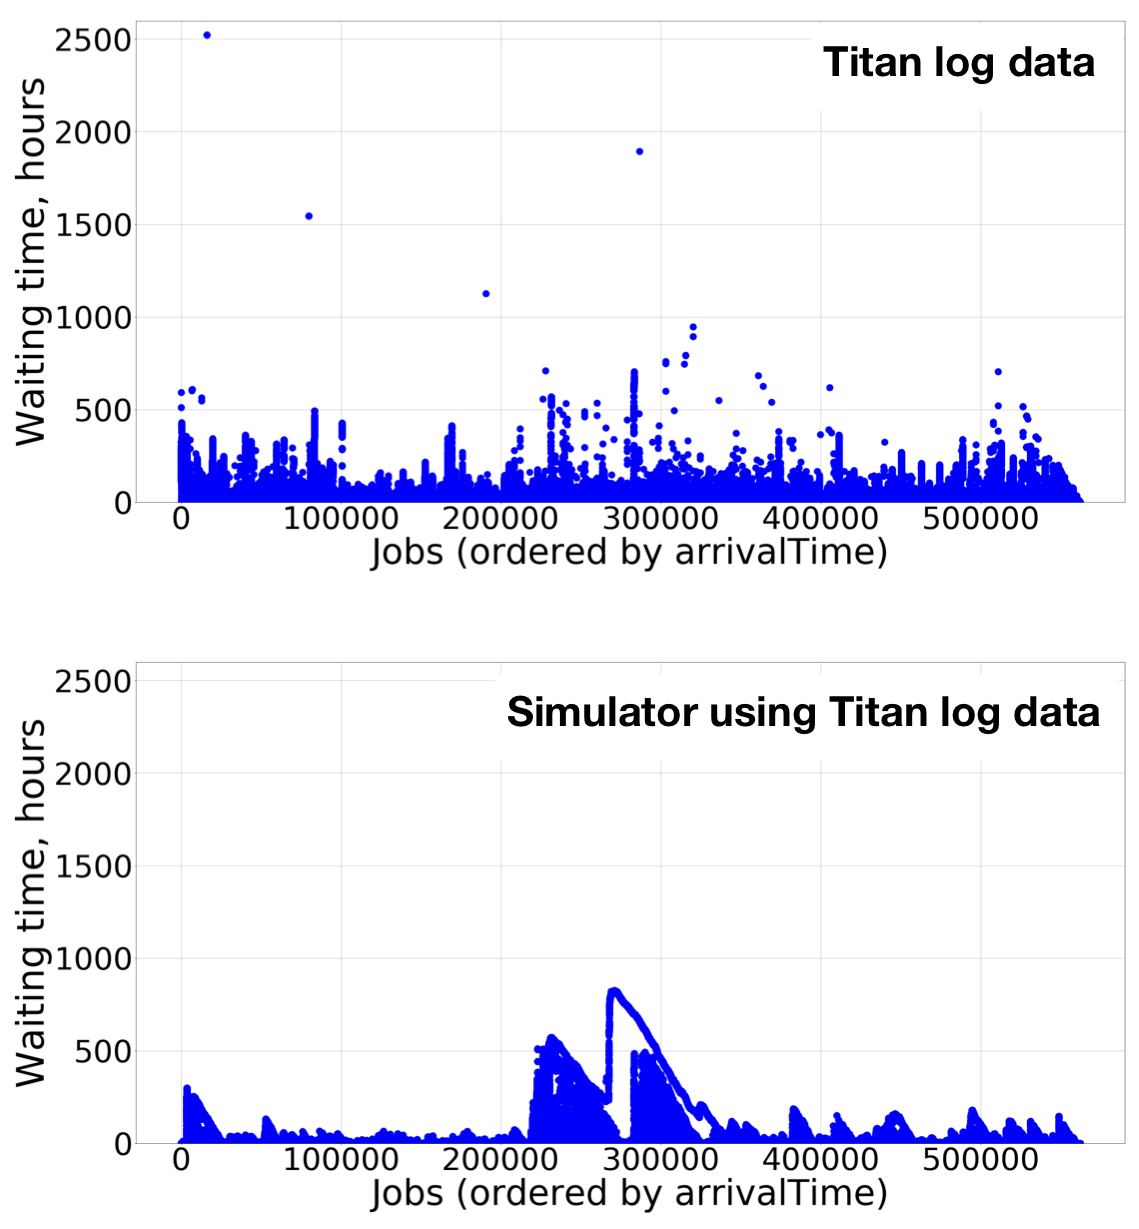
\includegraphics[width=0.45\textwidth]{pics/simulator-testing.png}
    \caption{Job waiting times based on Titan log data and Simulator log data with initial parameters from Titan log data (waiting time, hours - Titan: mean=6.21, std=29.77; Simulator: mean=30.51, std=97.34)}
    \label{fig-simulator-testing} 
\end{figure}

Figure~\ref{fig-simulator-load-1y} shows the load of the simulated nodes (i.e., the number of busy nodes at every simulated time unit, seconds) during the simulation process of jobs described earlier. The average utilization rate of the set of service nodes is 88.2 \%.

\begin{figure}
    \centering
    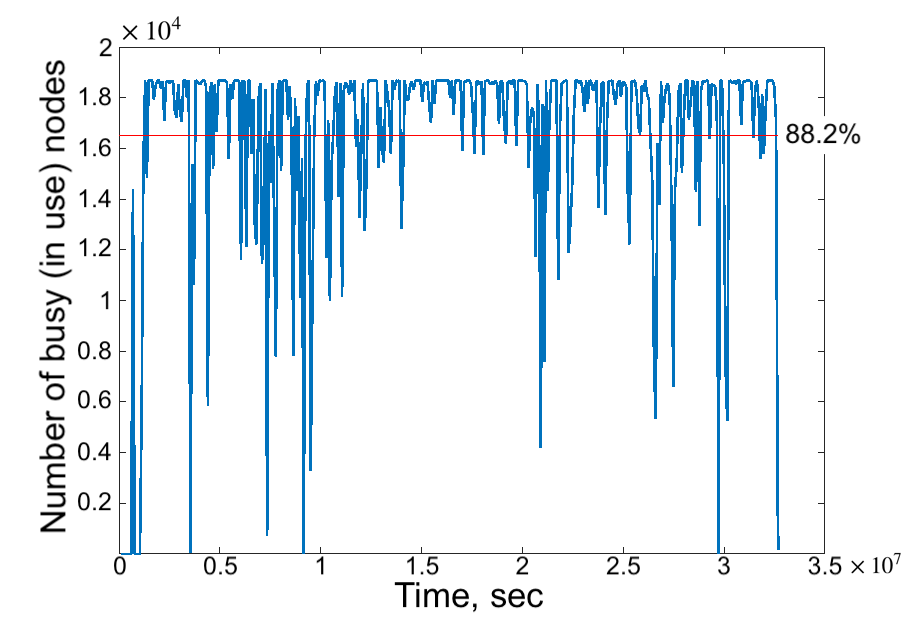
\includegraphics[width=0.45\textwidth]{pics/simulator-load-1y.png}
    \caption{The load of simulated service nodes (18,688 nodes)}
    \label{fig-simulator-load-1y} 
\end{figure}
